\documentclass[xcolor=table,dvipsnames,svgnames]{beamer}
% Author: alick<alick9188@gmail.com>

% This file is modified from a solution template for:

% - Giving a talk on some subject.
% - The talk is between 15min and 45min long.
% - Style is ornate.

% Copyright 2004 by Till Tantau <tantau@users.sourceforge.net>.
%
% In principle, this file can be redistributed and/or modified under
% the terms of the GNU Public License, version 2.
%
% However, this file is supposed to be a template to be modified
% for your own needs. For this reason, if you use this file as a
% template and not specifically distribute it as part of a another
% package/program, I grant the extra permission to freely copy and
% modify this file as you see fit and even to delete this copyright
% notice.

\mode<presentation>
{
  \usetheme[secheader]{Boadilla}
  \usefonttheme[onlymath]{serif}
  \setbeamercovered{transparent=5}
  \definecolor{thupurple}{HTML}{93278F}
  \definecolor{thudarkpurple}{HTML}{5C307D}
  \definecolor{thulightpurple}{HTML}{BC9BCC}
  \setbeamercolor*{structure}{fg=thupurple}
  \setbeamercolor*{palette primary}{fg=black,bg=thulightpurple}
  \setbeamercolor*{palette secondary}{fg=white,bg=thupurple}
  \setbeamercolor*{palette tertiary}{fg=white,bg=thudarkpurple}
  \setbeamercolor*{palette quaternary}{fg=white,bg=black}
}

\usepackage{graphicx}
\graphicspath{{fig/}}
\usepackage{listings}
\usepackage{xspace}
\usepackage{amsmath}
\usepackage{calligra}
\usepackage{cclicenses} % CC symbols
\usepackage{fontspec}
\usepackage[UTF8,nofonts]{ctex}
\usepackage{hologo}
\usepackage{colortbl}
\usepackage{hyperxmp}
\hypersetup{
pdfauthor={Alick Zhao},
pdfcopyright={Copyright (C) 2015 by Alick Zhao.
Licensed under CC-BY-SA 4.0. Some rights reserved.},
pdflicenseurl={http://creativecommons.org/licenses/by-sa/4.0/},
}

% xeCJK conf setup
\punctstyle{kaiming}
\renewcommand\CJKfamilydefault{\CJKsfdefault} % for slides

\setCJKmainfont[BoldFont={SimHei},
ItalicFont={KaiTi}]{SimSun}
\setCJKsansfont{WenQuanYi Micro Hei}
\setCJKmonofont{WenQuanYi Micro Hei Mono}

\setCJKfamilyfont{zhsong}{SimSun}
\setCJKfamilyfont{zhhei}{SimHei}
\setCJKfamilyfont{zhkai}{KaiTi}

\newcommand*{\songti}{\CJKfamily{zhsong}} % 宋体
\newcommand*{\heiti}{\CJKfamily{zhhei}}   % 黑体
\newcommand*{\kaishu}{\CJKfamily{zhkai}}  % 楷书

\newcommand{\BibTeX}{\hologo{BibTeX}}
\newcommand{\XeTeX}{\hologo{XeTeX}}
\newcommand{\pdfTeX}{\hologo{pdfTeX}}
\newcommand{\beamer}{\textsc{beamer}}
\def\TeXLive{\TeX{} Live\xspace}
\let\TL=\TeXLive
\newcommand{\ThuThesis}{\textsc{ThuThesis}\xspace}

% From thuthesis user guide.
\def\cmd#1{\texttt{\color{DarkBlue}\footnotesize $\backslash$#1}}
\def\env#1{\texttt{\color{DarkBlue}\footnotesize #1}}
\def\cmdxmp#1#2#3{\small{\texttt{\color{DarkBlue}$\backslash$#1}\{#2\}\hspace{1em}\\ $\Rightarrow$\hspace{1em} {#3}\par\vskip1em}}

% For debugging.
%\includeonlyframes{current}

\title
{\ThuThesis 最新动态}

\author[alick] % (optional, use only with lots of authors)
{赵涛\\ \texttt{alick9188@gmail.com}}

\institute[TUNA] % (optional, but mostly needed)
{
  清华大学电子系网络融合实验室
}
% - Use the \inst command only if there are several affiliations.
% - Keep it simple, no one is interested in your street address.

\date
{2015年5月21日}

\subject{ThuThesis, GitHub}

% If you wish to uncover everything in a step-wise fashion, uncomment
% the following command:

%\beamerdefaultoverlayspecification{<+->}

\lstset{basicstyle=\footnotesize\ttfamily,breaklines=true}
\hypersetup{
%pdfpagemode=FullScreen,
}

\logo{
\includegraphics[height=.15\textheight]{tuna-logo.pdf}}

\begin{document}

\begin{frame}
  \titlepage
\end{frame}

% Since this a solution template for a generic talk, very little can
% be said about how it should be structured. However, the talk length
% of between 15min and 45min and the theme suggest that you stick to
% the following rules:

% - Exactly two or three sections (other than the summary).
% - At *most* three subsections per section.
% - Talk about 30s to 2min per frame. So there should be between about
%   15 and 30 frames, all told.

\section{简介}

\lstMakeShortInline|

\begin{frame}{\ThuThesis}
  \framesubtitle{清华大学学位论文 \LaTeX{} 模板}
  \begin{itemize}
  \item 最早:王磊~(2004.4)
  \item 2005 年:薛瑞尼
  \item 上一发布版:\ThuThesis v4.6 (2011/10/22)
  \item 全面支持本科、硕士、博士、博士后论文格式
  \item 最新发布版:\ThuThesis v4.8.1 (2014/12/09)
  \end{itemize}
\end{frame}
\section{\ThuThesis 新版本}
\subsection{\ThuThesis 4.8.1}
\begin{frame}[fragile]{\ThuThesis 4.8.1}
  \begin{itemize}
    \item 基于 |ctexbook| 文档类
      \begin{itemize}
        \item 不再需要多记一种语法
        \item 不再支持 latex+dvips+ps2pdf 编译方式
        \item 字号命令保留,如 |\banxiaosi[1.3]|
      \end{itemize}
    \item 转向 UTF-8 字符编码,不再支持 GBK
    \item 硕士论文英文封面
    \item 各种BUG修正
      \begin{itemize}
        \item 本科生作者信息名称、关键词、页码字号、标题下划线等
      \end{itemize}
    \item 引入中文字体选择脚本 |zhfonts.py|
  \end{itemize}
\end{frame}

\subsection{\ThuThesis 4.8.2}
\begin{frame}[fragile]{\ThuThesis 4.8.2}
  \begin{itemize}
    \item BUG修正版本
      \begin{itemize}
        \item 避免 XeTeX 引擎下部分数学符号字体被自动调整成 CMR
        \item 修正(奇怪的)章节间距问题
        \item 修正学位论文中目录里节前缩进
        \item 修正定理标题为黑体
        \item 修正博士后简历页标题
        \item 参考文献支持电子文献类型 |online|
      \end{itemize}
  \end{itemize}
\end{frame}

\subsection{\ThuThesis 4.9}
\begin{frame}[fragile]{\ThuThesis 4.9}
  \begin{itemize}
    \item 固定字体设置,兼容 |ctex| 2.0
      \begin{itemize}
        \item 推荐中易六种字体
        \item 仍可以通过修改 |thufonts.def| 自定义字体
      \end{itemize}
    \item Makefile 缺省使用 latexmk 自动化编译
    \item 简历部分更符合格式指南和示例文件
      \begin{itemize}
        \item 引入新列表环境 |publications|、|achievements|
        \item |publications| 环境之间自动加空行
      \end{itemize}
  \end{itemize}
\end{frame}
\section{使用指南}
\begin{frame}{如何使用最新版本?}
      \begin{columns}
        \begin{column}{.7\textwidth}
  \begin{itemize}
    \item 下载最新版
      \begin{itemize}
        \item \url{https://github.com/xueruini/thuthesis}
        \item 右边栏
          \href{https://github.com/xueruini/thuthesis/archive/master.zip}%
          {Download ZIP} 按钮
        %\item Git 用户还可以直接克隆仓库
      \end{itemize}
  \end{itemize}
        \end{column}
        \begin{column}{.3\textwidth}
          \begin{figure}[htbp]
            \centering
            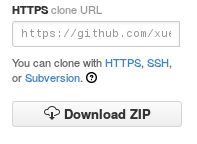
\includegraphics[width=.8\textwidth]{thuthesis-download.png}
          \end{figure}
        \end{column}
      \end{columns}
  \begin{itemize}
    \item 安装
      \begin{itemize}
        \item 解压缩看文档 \texttt{README.md}
        \item 模板文档类:(Xe)LaTeX 引擎处理 \texttt{thuthesis.ins} $\Rightarrow$
          \texttt{thuthesis.cls} 和 \texttt{thuthesis.cfg}
        \item 用户手册:latexmk 处理 \texttt{thuthesis.dtx} $\Rightarrow$
          \texttt{thuthesis.pdf}
        \item 论文示例:latexmk 处理 \texttt{main.tex} $\Rightarrow$
          \texttt{main.pdf}\\
          (或对 \texttt{main.tex} 执行一次 XeLaTeX,一次 BibTeX,再两次
          XeLaTeX)
        \item 可使用或参考附带的 Makefile
      \end{itemize}
  \end{itemize}
\end{frame}

\begin{frame}[fragile]{提醒}
  \begin{itemize}
  \item 参考文献不能为空
    \begin{itemize}
      \item 至少需要引用一篇参考文献
      \item 如果不需要参考文献,可将 |main.tex| 中 |\bib| 开头两行删除或注释
    \end{itemize}
  \item 同一字体勿重复安装
    \begin{itemize}
      \item 检查 |fc-list :lang=zh file family style > zhfonts.txt| 命令输出
    \end{itemize}
  \item 过长的 URL
    \begin{itemize}
      \item URL 缩短服务
      \item 定制 URL 断行规则:|\PassOptionsToPackage{hyphens}{url}|
    \end{itemize}
  \item 附录中自动生成参考文献列表
    \begin{itemize}
      \item 现有基于\href{https://github.com/linhr/thuappendixbib}{chapterbib}%
        的临时解决方案
      \item 基于 biblatex 的方案有待研究
    \end{itemize}
  \end{itemize}
\end{frame}

\begin{frame}{遇到问题}
\begin{itemize}
  \item \href{https://github.com/xueruini/thuthesis/issues}{GitHub Issues} 提问
  \item \TeX @newsmth 查找或发文
  \item \href{http://groups.google.com/group/thuthesis}\ThuThesis{} Google Group 发问
\end{itemize}
\end{frame}


\begin{frame}{参与贡献}
\begin{itemize}
\item 错误反馈与改进建议:GitHub Issues
\item 出力维护:代码更新整理
\item 科普、答疑
\end{itemize}
\end{frame}

\section*{附录}

\begin{frame}
  \begin{itemize}
    \item 本幻灯片基于:\url{https://github.com/alick/thulib-latex-talk}
    \item 许可证:CC BY-SA 4.0 Unported \cc\ccby\ccsa
  \end{itemize}
\end{frame}

\begin{frame}
  \begin{center}
    {\Huge\calligra Thank you!}
  \end{center}
  \begin{figure}[htbp]
    \centering
    
\includegraphics[height=.3\textheight]{url.pdf}
  \end{figure}
\end{frame}

\end{document}
%%% vim: set sw=2 isk+=\: et tw=80 cc=+1 formatoptions+=mM:
